\chapter{Deployment in the Field}\label{chap:imp}
	In this chapter, we detail the design and deployment of a modified K-HAS in the Malaysian rainforest. We also highlight the issues we experienced deploying the architecture in a humid, dense rainforest for use by those without domain knowledge of WSNs.
	
	Experiments carried out in the rainforest had already shown that the range of wireless communications could be reduced by up to 80\% and we expected that the lifetime of nodes in such conditions would be affected, based on experiments explained in Section \ref{tech:wireless}.
	
	Yearly visits were made to the Danau Girang Field Centre (DGFC) to test different nodes, gather knowledge and trial iterations of K-HAS. The first visit showed us just how much the rainforest affected communications, but also allowed us to gather knowledge from researchers and cameras that had previously been deployed. Subsequent visits were then used to test our own nodes and software, based on the knowledge we had gained from the first visit, explained in Section \ref{tech:wireless}. We developed K-HAS with a view to deploying it in Malaysia, however, it soon became clear that our design was  beyond what was currently available, as well as the time constraints.
	
	Developing a camera with both wireless and processing capabilities, as well as being waterproof, proved to a be an extremely difficult task, while wireless wildlife cameras were already commercially available with range much higher than what our experiments had yielded. This could be because of their test environments being places such as American forest with less dense foliage, lower canopies and much lower humidity and using wireless technologies that are not licensed for worldwide use. For our own node designs, we attempted to use various node types connected to a camera, such as the Raspberry Pi and Waspmote nodes; both yielded problems with mounting an SD card that was readable by both camera and node. At the time, we were unable to create a camera combined with a node that could be left untouched for months at a time in a rainforest.
	
	However, we still needed to implement a network to evaluate our approach, thus we developed a modification to the K-HAS that utilised the latest commercially available hardware to provide an architecture that provides similar capabilities. Because these changes were made due to issues with deployment in Danau Girang, we chose to name it LORIS, after a famous animal in Malaysia. A Slow Loris is a small, nocturnal primate commonly found in South and Southeast Asia but in our context it is an acronym that stands for Local-knowledge Ontology-based Remote-sensing Informatics System.
	
	LORIS has been developed specifically for the Malaysian rainforest, our motivating scenario and, as such, much of the hardware and software has been implemented to reflect this.
	
	The rest of this chapter is structured as follows. Section \ref{loris:arch} highlights the changes we had to make from K-HAS and explains the hardware used at each tier. Section \ref{loris:dep} explains how we planned and deployed the network. Section \ref{loris:res} details the results from the deployment in Malaysia and Section \ref{loris:conc} concludes the chapter with a summary of our results.
	
	\section{ Deployment Architecture}\label{loris:arch}
		The aim of LORIS was to keep as much of the architecture of K-HAS as possible and reuse the ontology without the need for modification; serving as a form of validation. In order to do this, we identified the tiers of the network that could be deployed in the rainforest, given the hardware and wireless constraints, and the areas that needed to be addressed. Regular power and cheap computers with good knowledge-processing capabilities meant that DA nodes were simple to deploy and, with the growth of powerful microcomputers like the Raspberry Pi, DP nodes were also in abundance. However, finding a reliable camera that could integrate with a node capable of processing observations that was also reliable enough to withstand the humid rainforest proved to be difficult.
		
		\subsection{Data Collection}
				Experiments were run yearly in Malaysia to test the performance of variations of hardware. As covered in Section \ref{tech:wifi}, the first year involved testing the range of Wi-Fi with an IGEP board. The limited range of 30m meant that, despite the high transfer rate, it was not possible. Wi-Fi was not designed for use in resource-constrained sensors, so the power consumption of the radio meant that it limited the lifetime of the node.
				
				The following year, we used the Digimesh protocol, explained in Section \ref{tech:range:digimesh}, which provided a longer range and was developed for use in sensor networks.  While the range was suitable for the rainforest, it was not as much as we had anticipated. The other difficulty proved in mounting an SD card on two devices at the same time, the existing wildlife cameras and our Waspmote nodes, without causing corruption from read/write clashes.
				
				From these experiments, we began to look into commercial alternatives that combined both the node and the camera. The most usable solution we found was the Raspberry Pi coupled with a camera attachment \cite{Sarajevo2014}, but it was not ready for use in the Malaysian rainforest or to be used for an extended unsupervised period. Existing wildlife manufacturers were then looked into and we found that wireless cameras had been manufactured, but they had no local processing capabilities and had not been used much in research. Based on these findings, we used Buckeye X7R cameras \cite{Buckeye}. Using the same Digimesh protocol as the Waspmote, they had a tested range of 1 mile and their casing had been developed to withstand harsh environments. The 1 mile range was tested in a more open woodland in the US but the higher quality components used, as well as their modifiable antenna supported our theory that we would achieve better range with their cameras.
				
				We expected to achieve around 800m of range and these proved to be suitable DC node replacements, despite the fact that we had to forgo local processing or the storage of any local knowledge.
		\subsection{Data Processing and Aggregation}
				Because our DC nodes were wildlife cameras that did not have any knowledge processing capabilities, and because our DC node sites were near enough to the field centre, we combined the DP and DA nodes into one machine stored at DGFC, that contained both a Digimesh radio and an Internet connection. The benefit of using commercial grade hardware was the software that accompanied it; remote management and configuration software allowed users to modify the settings on each camera, as well as handling the retrieval of images from every node deployed. EXIF tags written to images could be modified, as well as how many images were captured for each observation. The software had been created to be used by those without any specialist knowledge and was easily used by researchers in the field centre.
				
				Each observation was saved into a directory that matched the ID of the camera it originated from and this meant that the existing software used in K-HAS could be used without modification. Sensor middleware, such as GSN, is running on the same machine and virtual sensors listen for changes in each directory; where each virtual sensor represents a deployed camera.
				
				When new observations are detected, Drools runs on the images to start metadata and EXIF processing. Some rules had already been extracted from the processing of 120,000 images collected from our yearly visits to DGFC; other rules had to be added by users of the WSN. When an observation had been processed, rules were run once again to determine if a match could be made to existing projects and, if so, who should be notified.
				
				The web interface for classifying and viewing all observations was accessible by those within DGFC, as well as uploading rule files and new locations. Using this interface proved to be easier for those without a WSN background and the GSN interface had a steeper learning curve.	Figure \ref{fig:loris} shows the basic metadata of an observation, outlining where it was captured and when; as well as the images themselves.
				
				\begin{figure}[h]
				\centering
				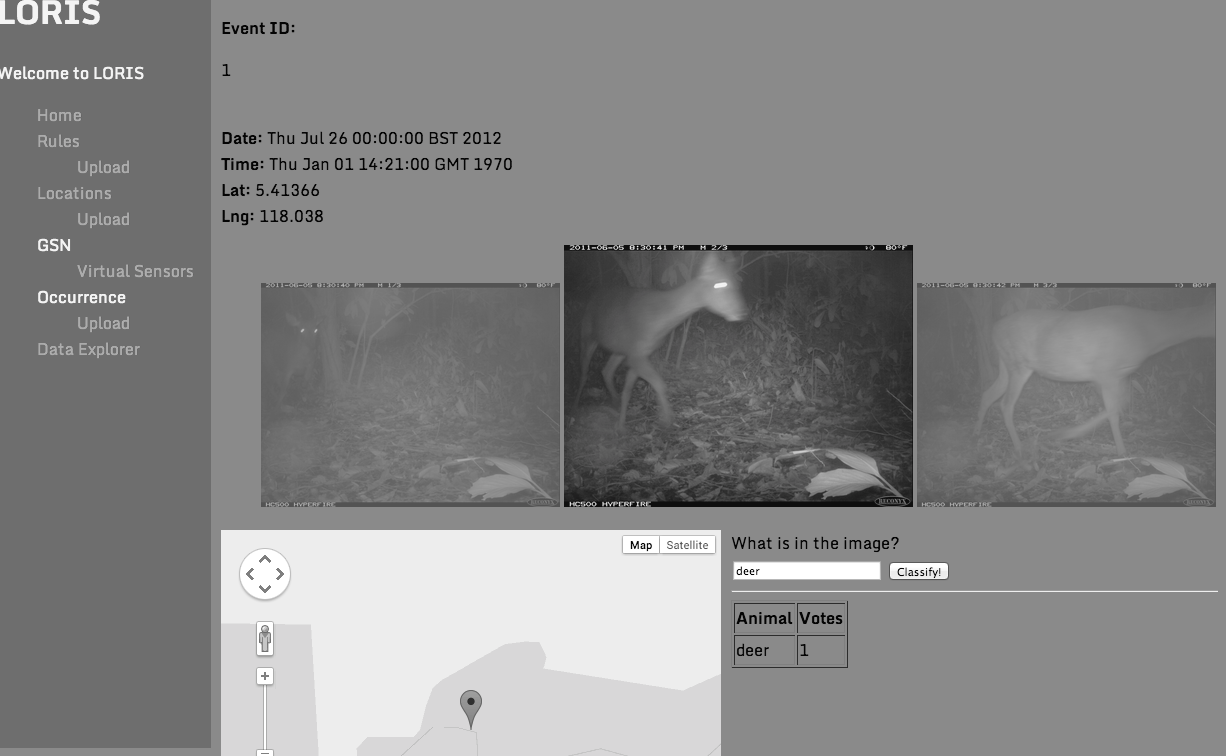
\includegraphics[width=\textwidth]{Chap6/figures/loris}
				\caption{LORIS Web Interface}
				\label{fig:loris}
				\end{figure}
				
	\section{Deployment}\label{loris:dep}
		In June of 2013, a three week visit was made to Danau Gurang, with three Buckeye cameras and the software required to deploy LORIS. The network was first tested within the field centre and one of the Buckeye cameras had been broken during transport, giving us only two cameras. Due to the protected nature of the forest, we were unable to nail any cables to trees to use the high gain antenna and it was not possible to use the cables without first securing them, because animals tampering with cameras was a common occurrence.
		
		For the initial week of the deployment, we wanted to test the robustness of the network before focussing on the data. This meant placing the cameras in locations where they would be triggered often and in an area where they would be affected by rainfall and humidity. Figure \ref{cam_locs} shows the locations of the cameras during both of the weeks that it was deployed. Buckeye 1 was deployed for the first week along the main path leading to the field centre from the river, this experienced the most traffic due to the number of researchers present at the time. 
	
	    \begin{figure}[h]
	    \centering
		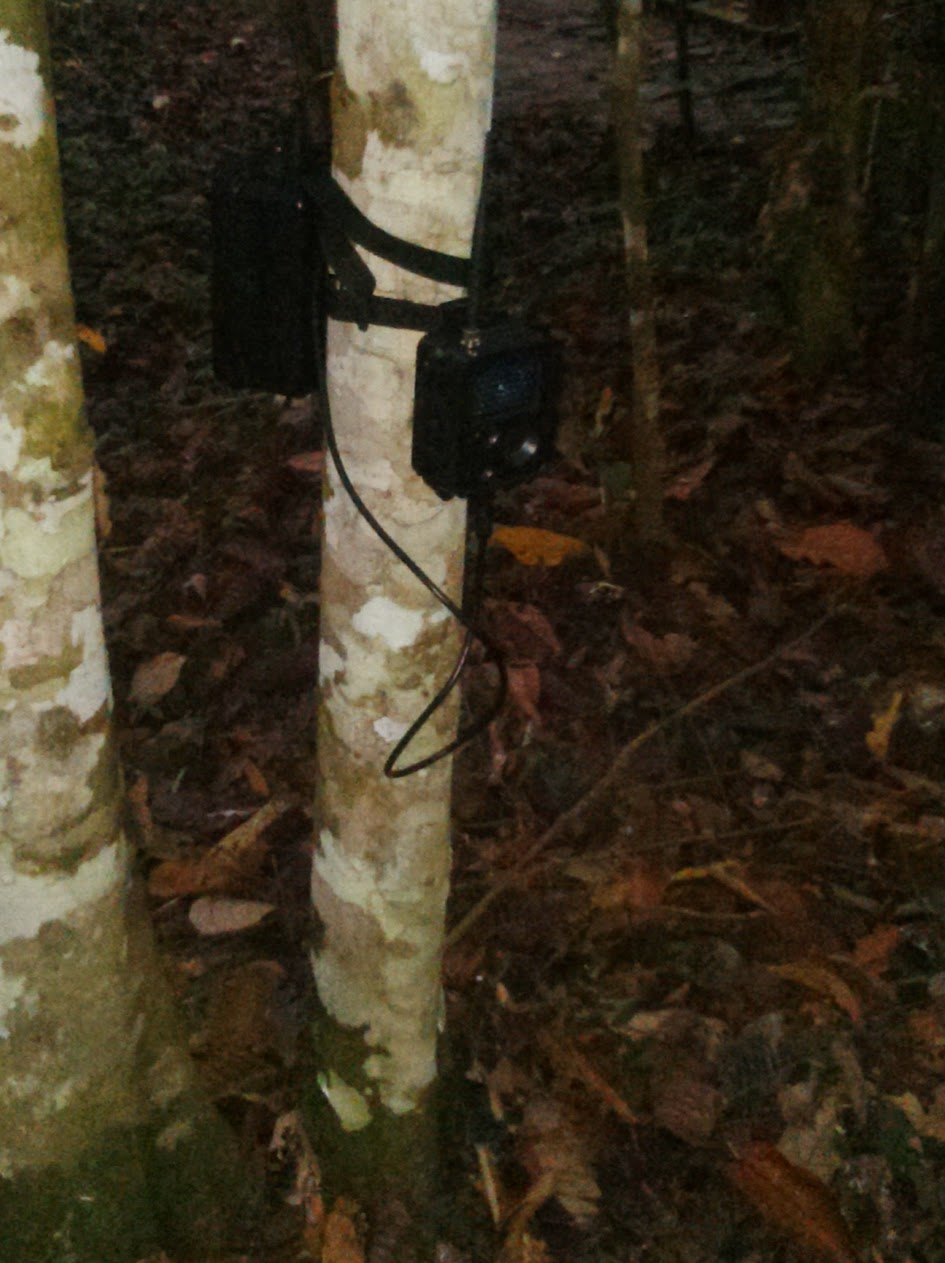
\includegraphics[width=\textwidth]{Chap6/figures/buckeye}
	    \caption{Camera Locations Around Danau Girang}
	    \label{cam_locs}
	    \end{figure}
	
		\subsection{Direct Connection}
		For six days, we tested two Buckeye cameras that were near enough to the field centre to maintain an active connection to the base station. This meant that no hopping was involved and cameras were not reliant on each other to transmit images. Buckeye 1 was placed on a main path that guaranteed human foot traffic and Buckeye 3 was placed on a trail in the forest that, while experiencing minimal foot traffic, was expected to yield small mammals and birds.
		
		For the duration of the six days, the cameras did not report a drop in battery levels and a total of 1076 images were sent. Buckeye 1 was in a more open environment, despite being further away, and average speeds of 4KB/s were achieved. 
		
		Transmissions from Buckeye 3 were significantly hampered by the dense forest that it was surrounded by, as well as the fact that a low-gain antenna was used. We also speculate that the field centre itself acted as a barrier to the signal, as the base station was located on the opposite end. Because of this, we experienced an average speed of 1.2KB/s, taking around three minutes to receive an image. This is consistent with experiments conducted in previous years where dense, humid forest has led to a decreased range of, up to, 78\%. Lower frequencies do experience a longer range, but the data rate is significantly impacted.
		
		\subsection{1-Hop Network}
		For a further five days, Buckeye 1 was moved further into the forest and Buckeye 3 was set up as a routing camera that forwarded images onto the base station, 63 images were taken during this period.
		
		The location of the moved camera is also shown in Figure \ref{cam_locs}. As was expected, the traffic of the network reduced significantly when the cameras were moved from the main path, with almost all 63 pictures being of animals. Due to animals moving a lot faster than humans, the number of pictures taken per trigger was increased to two, this would ensure network traffic was not overwhelming while increasing the chance of capturing the subject.
		
		Surprisingly, the speed of transmission from Buckeye 1 was faster than Buckeye 3, despite being routed through it, with an average speeds of 1.8KB/s.				
		\section{Results}\label{loris:res}
		Deploying a network for two weeks is not a robust experiment and does not show that LORIS can withstand months of running without human intervention. However, it does serve as a proof of concept that, using commercial hardware, a modified K-HAS network can be implemented and utilise the knowledge of its environment.
		
		The pictures of humans from the first six days are not of use for the current motivating scenario, focussed on animals in the rainforest corridor, but one could see this network also being tasked to warn the authorities of hunters in restricted areas of the rainforest. However, the images we have of animals, while few are animals of interest due to the proximity of the cameras to humans, were processed and used to create templates for future observations. 
		
		    \begin{figure}[h]
		    \centering
			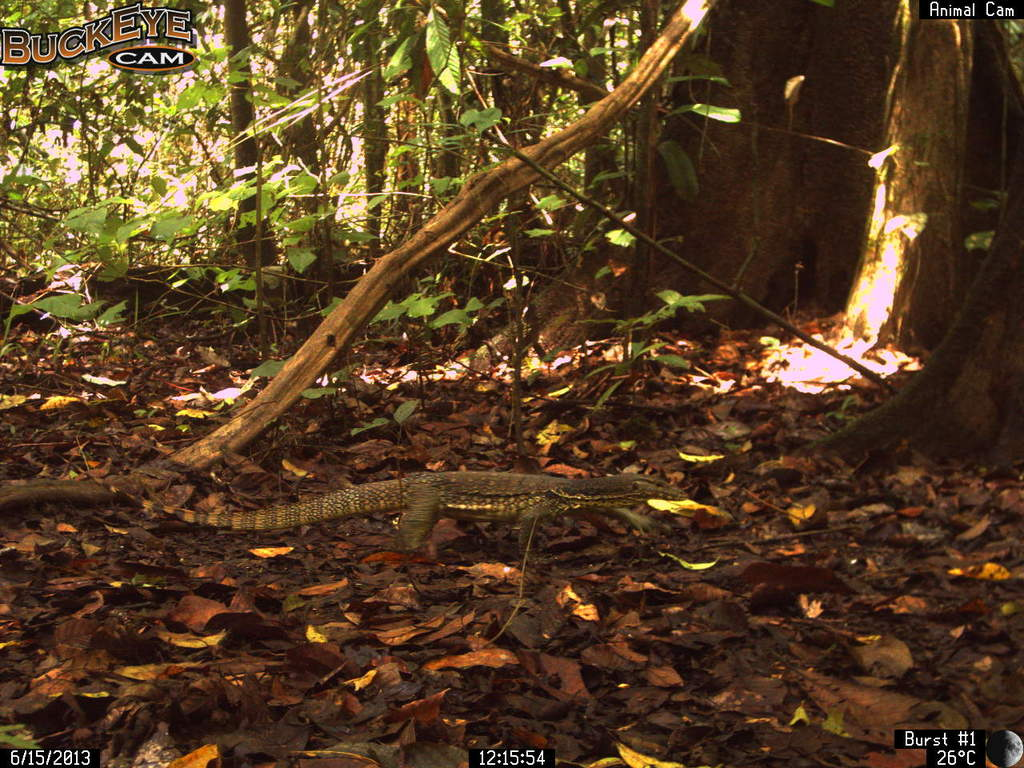
\includegraphics[width=\textwidth]{Chap6/figures/buckeye_img}
		    \caption{First Image of Lizard by Buckeye 3}
		    \label{buckeye_img}
		    \end{figure}
		
		More interestingly, we were able to infer further rules from the short deployment that helped us to narrow down the choice of animals to match to based on the time of day and location. For example, Figure \ref{buckeye_img} shows a lizard crossing the path of Buckeye 3 in the middle of the day and Figure \ref{buckeye_img_2} shows the lizard walking past in early afternoon on a different day. This allows us to encode a window of time  in which the lizard is more likely to appear onto the static knowledge base of DC nodes or, in the case of LORIS, onto the DA/DP node. Images an hour later were captured by the camera, showing the lizard walking in the opposite direction. While this was not every day, and the deployment time was too short to establish a pattern, it does help us to infer that a lizard passing by in early afternoon is likely to walk the same path approximately an hour later.
		
		    \begin{figure}[h]
		    \centering
			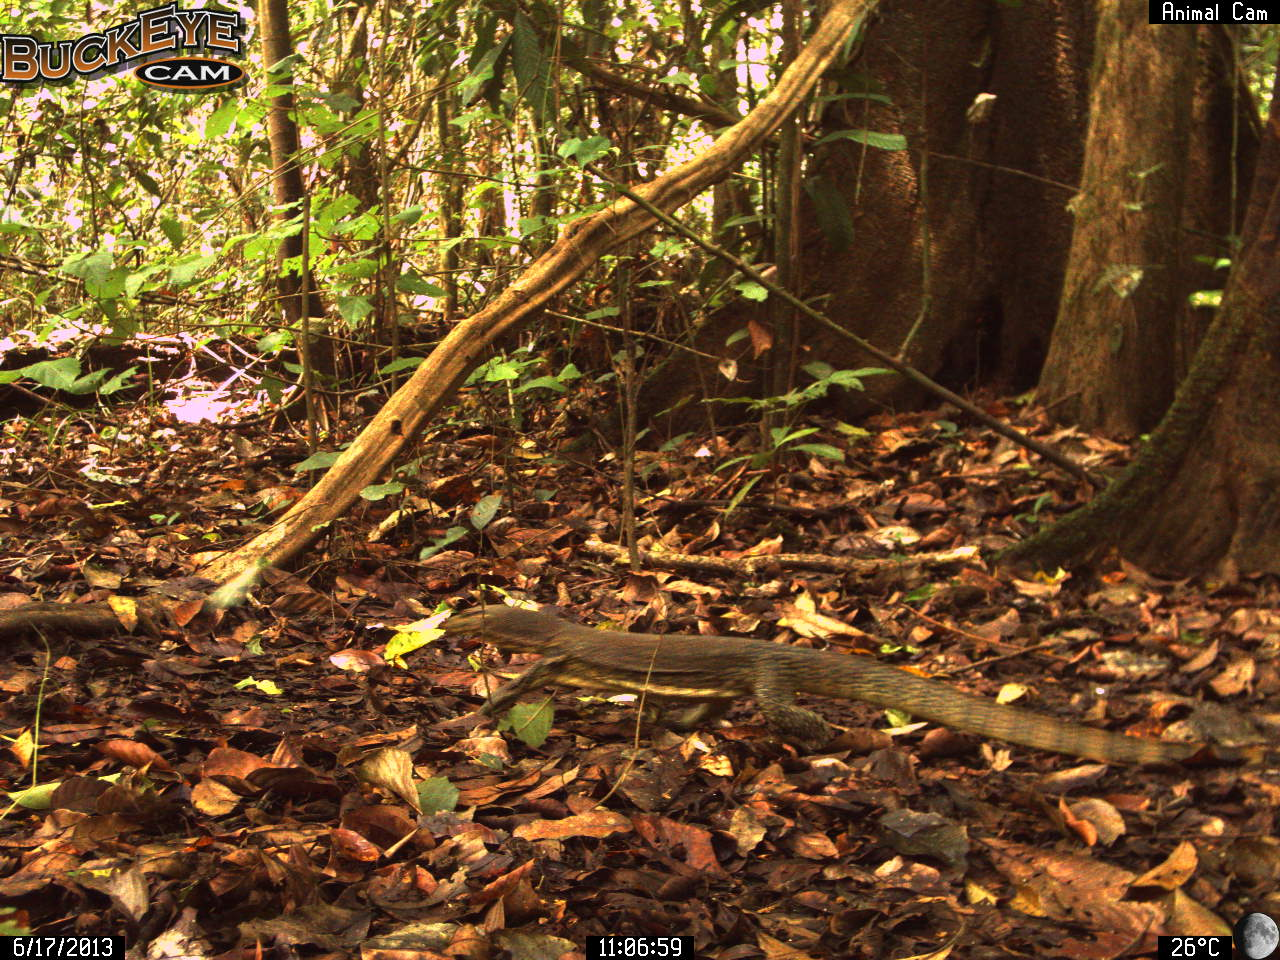
\includegraphics[width=\textwidth]{Chap6/figures/buckeye_img_2}
		    \caption{Second Image of Lizard by Buckeye 3}
		    \label{buckeye_img_2}
		    \end{figure}
	
	\section{Rules}
		This section explains the rules used in LORIS and K-HAS in more detail, to highlight how classifications are made as well as how nodes in the network are monitored. Any examples made here relate to our motivating scenario. The rules on each node are a vital way of encoding local knowledge and a practical use to show how local knowledge, from users or previously sensed data, can be used classify newly sensed data.
		
		As highlighted in Section \ref{arch:kb}, K-HAS uses the Drools rule engine, a Java based rule management system that uses forward chaining based inference. Forward chaining starts with some data, in our case a set of images, and uses inference rules to extract more data. We use this method to make meaningful inferences from properties of the sensed data. For example, an image taken at 8pm could be run through Drools and an inference rule will tell the system to start by looking for nocturnal animals.
		
% 		\subsection{Data Collection}			
% 		As explained in Section \ref{khas:dc}, DC nodes are unable to run the Drools engine and instead utilise static rules that are encoded at the time of deployment. Instead of utilising forward chaining to draw a single conclusion, these rules are executed one by one and the outcome of one does not affect the outcome of another. An example of such rules could be a rule to determine the time of day that an image was captured (such as morning, afternoon, evening or night) or a rule to determine what animals it is more likely to be based on the temperature and location of the node, shown in Listing \ref{lst:dcrule}. No rule engine is used by the DC node and the rules are executed in the code before the observation is archived and sent on.
		
% \begin{lstlisting}[caption=Encoded Data Collection Rule, label=lst:dcrule, breaklines=true]
% 	if img.temp > 32 && img.temp < 38 then
% 	classification.potentialAnimals = [clouded_leopard, malay_civet, sun_bear]
% 	if img.time > 1800 && img.time < 0500 then
% 	classification.animalBehaviour = nocturnal
% \end{lstlisting}
	
	\subsection{Data Processing and Data Aggregation}
		The increased knowledge-processing capabilities allow DP nodes to run a complete implementation of Drools, this means that forward chaining can be used and the knowledge base is dynamic, i.e. it can be updated whilst the network is deployed. 
		
		Rules are written in \textit{drl} files that are loaded into a knowledge session. Sessions, as well as the firing of rules, are handled by the Java code. The benefit of using Drools with a Java based middleware, such as GSN, allows the simple integration of the two technologies, allowing a sensor class in GSN to insert an archive into the session and run the rules. When sensed data is received from a DC node, it is unarchived and Drools is run on the DwC files describing the original observation, the metadata, the originating DC node and the knowledge base of the DP node.
		
		Listing \ref{drools:dp} shows a psuedocode example of some more simple rules that could be contained within the knowledge base, a full listing is in Appendix \ref{appendix:drools}. In a rules file, existing local knowledge is used with the properties of a new observation to infer the contents and then update the DwC archive, or return suggestions as to what the contents may be. For example, the sample rule uses the location ID of the camera to check if it is near a plantation and uses local knowledge of the area and global knowledge of the time to infer that the image may contain a sun bear or malay civet, based on the knowledge that they have been known to forage in the plantation at night when there are no humans. This rule maps to the terms defined in the ontology (Chapter \ref{chap:ont}) where the individual is a sun bear or a malay civet, the evidence is an image and the occurrence is the DwC archive created by the triggering of a DC node.
		
		\vspace{\baselineskip}
		\begin{lstlisting}[breaklines=true, caption={Pseudocode of a Drools Rules File}, label={drools:dp}]
rule "Plantation night"
	when New_Sensed_Data
		if location of node is Plantation and time of day is night
			write to file set.CSV
				dateIdentified = \today
				scientificName = sun bear
				identifiedBy = node ID
			Print "Likely a sun bear or malay civet"
				\end{lstlisting}
		
		These rules are very simple and only scrape the surface of the local knowledge that can be utilised, as well as how DwC archives can be effectively used to carry the data of these inferences, but it does show that Drools is a powerful rule engine and that these rules can be extended further to make full use of the knowledge base. 
		
		DA nodes use the same rule engine as DP nodes but rules are used for the post-processing of Darwin Core archives. For example, when a classified archive is received from a DP node, Drools is run to check if the classification matches an existing project. If it does, then it searches for those that are subscribed to the project and notifies them via their selected medium. Drools can also be used to monitor the nodes deployed in the network and check their status. Rules are run to check for archives from DC nodes and, if a node has not sent an archive in a set number of days, then administrators are informed that it may have run out of battery.
		
		More importantly, rules are vital for the exchange of knowledge between nodes in the network. If a user classifies an observation on a DA node, then rules are fired that identify the DP node that sent it and update the knowledge base, on the original DP, so that the image template it uses in future classification matches the one identified by the user.
		
		\subsection{Existing Data}
			Throughout our visits to Danau Girang, we collected local knowledge through field work and interviews with the researchers based at Danau Girang. As well as this, we collected classifications made by the researchers for images that had been taken during camera deployment. Using these data, we have extracted patterns in animal movements in order to create some basic rules for the DC and DP nodes. In this section, we will describe the data we have and the methods used to extract rules.
			
			\subsubsection{Semi Structured Interviews}
			On our final visit to Danau Girang, we designed a set of 14 semi structured interview questions that we asked to ten researchers based at the field centre, with the majority working on different projects. We used these questions to gain insight into common trends between projects and patterns recorded about the animal subjects. A subset of the questions have been listed below:
			
			\begin{itemize}
				\item What species are you looking at?
				\item Do you have specific sites that you look into?
				\item What specifics do you know about the target species?
				\item Do others use your research? If so, how?
			\end{itemize}
			
			These questions have been designed to be as open as possible to allow the interviewees to provide as much detail as they wish, or even transition to a different topic. The interviews were recorded and later transcribed to text. We then used a software package called Dedoose \cite{dedoose2012web}, which is an online tool that is used for performing qualitative analysis on text based documents. Uploading our documents to the service allowed us to manually review the responses to each question and highlight, or `tag', excerpts of interest and link to other excerpts that had either been mentioned by another interviewee; or were related to other comments. Each excerpt was tagged with the subject it was discussing, for example, a comment on the accessibility of an area of the forest during certain times of the year were tagged as \textit{local knowledge}. The excerpts were combined and exported into a CSV file that detailed who the interviewee was, the content of the excerpt and the tag. Appendix \ref{appendix:interview} shows an interview transcript and Appendix \ref{appendix:interview:extract} provides an extract of a file once it has been annotated within Dedoose.
			
			This method allowed us to gain knowledge we would not have learnt from our short time at the field centre, these face to face sessions gave us insight into patterns and observations that had been made by researchers who have been based at Danau Girang for many years. An example of this is the global knowledge of the sleeping patterns of Clouded Leopards. It is widely accepted that they are nocturnal however, the camera trapping project has shown that their sleeping patterns around Danau Girang do not support this and they have been seen throughout the day and night. This could be due to the human impact, availability of prey or even the climate of the area, but, if researchers had just used this global knowledge then they would have seen fewer Clouded Leopards. Similarly, if we had used a rule to only look for Clouded Leopards at night, then a lot of images would have been misclassified. While it cannot be directly encoded as a local knowledge rule to constantly look out for clouded leopards, this is an example of local knowledge overriding global knowledge.

			While we were not able to construct a full set of rules from these findings, the results have provided support for patterns extracted from existing data that has been classified by researchers, which we discuss further in the next section. 
			
			\subsubsection{Existing Data}
			When images are manually collected at Danau Girang, researchers process each image set and they have recently been recording the classifications. However, these classifications are only being recorded for currently ongoing projects and other images are ignored. During one of our visits, we collected a CSV file of 2650 confirmed classifications made by researchers. The data had not been cleaned and multiple users had used different names for the same species, we cleaned the data manually and matched it with the images in our database.
			We then used the classifications for each species to determine any patterns by analysing the details recorded for each observation, which are listed below:
			\begin{itemize}
				\item Time
				\item Date
				\item Location
				\item Temperature
				\item Moonphase
				\item Classification
			\end{itemize}
			
			SQL queries provided these details for each species and we recorded patterns that could be identified. For example, if a Samba Deer was only spotted between the hours of 7pm and 4am then we could write a rule that the species is nocturnal. More detailed rules can be created if there are patterns across multiple details. A species that is only spotted in two of the twenty sites between the hours of 7pm and 4am means that nodes with local knowledge can make accurate classifications without the need for image processing. However, these rules are based on large amounts of data collected from an active, or previous, deployment. DC nodes in their early deployment stages would not have the data to make such detailed rules.

				\begin{lstlisting}[breaklines=true, caption={Example Rule created from Existing Data}, label={imp:lst:rule1}]
if TIME > 1500 and TEMP <= 26:
    if TIME < 0000:
        if MOONPHASE <= 2:
            CLASSIFICATION = GOAT (25\% chance)
        if MOONPHASE > 2:
            if DATE in JAN:
                CLASSIFICATION = HUNTER (2.6\% chance)
				\end{lstlisting}
			
			Using the Weka package, we constructed a J48 decision tree and used the resulting model to create a collection of simple rules that could be run on a DC node. Figure \ref{imp:lst:rule1} shows a rule that was created from the output. This rule checks the time of capture for the observation, the temperature and the moonphase; which has been converted into a numeric value. If the temperature is less than 26 degrees and the time is between 3pm and midnight, then there is a 25\% chance of the classification being a goat. The if-statements are executed in order and the classification that matches the properties of the observation, and has the highest percentage chance, is forwarded to a DP node.
            
            Because the features used to generate the rules are available in every observation, and do not require any external information, DC nodes are able to process the series of if-statements quickly. This method of knowledge-processing comes at the cost of accuracy, when compared to using existing data, image processing and/or a dynamic knowledge base, but the speed and simplicity of these rules mean that they can be used by almost any node, regardless of computational capability.

		
	\section{Conclusion}\label{loris:conc}
	 K-HAS was developed, with the motivating scenario in mind, as an ideal, general-purpose network architecture that is able to utilise the knowledge of its environment. However, experiments to support the design and deployment of such a network within the timeframe of this PhD showed that the current technology was not ready to support a network that would run without human intervention for extended periods. LORIS is our more specialised, cut down approach that can be implemented using commercial hardware that is readily available, as well as software that we have open-sourced. 
	
	Our deployment in Malaysia has shown that local knowledge can assist with classifications and can be gained from even a few images collected within the first few days of deployment. Ideally, we would like to leave this network running for an extended period to infer rules from the sensed data and test the reliability of the network in harsh conditions. From both the visit and the deployment, we have offered evidence for the existence of local knowledge and provided a method that can be used to extract it from field experts. 
    
        The rules extracted from the interviews and classified data we collected while deploying LORIS can be used as a static knowledge base for DC nodes in the K-HAS architecture, or as the basic starting knowledge base for the DA node in LORIS. As more classifications are made to new sensed data, this same process can be used to create new rules for previously unrecorded classifications, as well as refine existing rules. 
	
	LORIS has shown that local knowledge can be used to enrich sensed data, and automate classification, when it has been received at the field centre, but we  maintain that K-HAS' aim of pushing local knowledge right out to the edge of the network makes a network more effective and allows for a more timely delivery of important sensed data.  The main drawback of LORIS is that it relies on the chronological delivery mechanism used by the commercial cameras, whereas K-HAS can improve this mechanism by sending the data that it infers to be of a higher importance, rather than what was simply captured first.